\subsection{Shared properties and indiscernibility}
\label{sec:indiscernibility}

When we look at the triples that constitute a set of identity relations,
  we see that all links look the same.
But when we take the triples in which the subject and object terms occur
  into account, we see that within the identity relation there may be
  different subrelations that we can identify in terms of the predicates
  that occur in the schema.

For instance, in the IIMB dataset there are some identical resources that
  share the property \verb|IIMBTBOX:spoken_in|, while other pairs share
  the property \verb|IIMBTBOX:form_of_government|.
The set of pairs of resources that are spoken in the same language may even
  be disjoint from the set of pairs of resources that have the same
  form of government.

Note that we are not only interested in the properties that resources share
  with one other (e.g., where they are spoken, or which form of government
  they have), but we are also interested in resource pairs that share
  the same sharing properties.
We can thus identify subsets of an identity relation based on differences
  in the sets of predicate path maps relative to which they take resources
  to be \emph{indiscernible} from one another.

In the example above, one subset of the identity relation does not discern
  resources that are spoken in the same language, whereas another subset
  of the identity relation does not discern resources that have the same
  form of government.

We say that two resources are indiscernible with respect to
  a set of predicate path maps $P \subset P_G^n$
  in case they share the same properties denoted by those ppms
  (def. \ref{def:resource_indiscernability}).\footnote{
    $P$ must be closed under the identity relation, i.e.,
    \begin{equation*}
      cl_{\sim}(P) = \bigcup_{\tuple{\range{p_1}{p_n}} \in P}\nolimits (
        [p_1]_{\sim} \times \ldots \times [p_n]_{\sim}
      )
    \end{equation*}}
We say that two resource pairs are indiscernible
  in case both pairs are indiscernible for the same
  $P^* \subseteq \mathcal{P}(P_G^n)$
  (def. \ref{pair indiscernibility}).\footnote{
    In order to assertain that $f_p(x)$ and $f_p(y)$ denote
      the same set of resources, identity does not suffice.
      $\approx$ gives a special treatment for blank nodes and
      typed literals (skipped here for brevity).
  }

\small
\begin{definition}[Indiscernibility]
\begin{align}
\label{def:resource_indiscernability}
\mathit{IND}(P) \,=\,
  \setdef{
    \pair{x}{y} \in S_G^2
  }{
    \forall_{p \in cl_{\sim}(P)} f_p(x) \approx f_p(y)
  }
\\
\label{pair indiscernibility}
\mathit{IND}(P^*) \,=\,
  \setdef{
    \pair{\pair{x_1}{y_1}}{\pair{x_2}{y_2}} \in (S_G^2)^2
  }{\\
    \forall_{P \in P^*}
        \pair{x_1}{y_1} \in \mathit{IND}(P)
      \leftrightarrow 
        \pair{x_2}{y_2} \in \mathit{IND}(P)
  }\nonumber
\end{align}
\end{definition}
\normalsize

\noindent As explained above, for a given set of identity pairs there
  may be multiple pairs that have the same shared properties.
These sets of predicates that are shared across resource pairs are
  considered to give a description of a specific subrelation of
  the identity relation.

According to the standard definition,
  identical resources are indiscernible with respect to all properties.
We take a given set of identity pairs and partition it into subsets which
  we can describe as being $cl_{\sim}(P)$-indiscernible,
  for $P \subseteq P_G^n$.

Fig. 1 shows an example
  of a discernibility partitioning for a given identity relation.

\begin{comment}
\begin{figure*}
\label{fig:iimb_example}
\centering
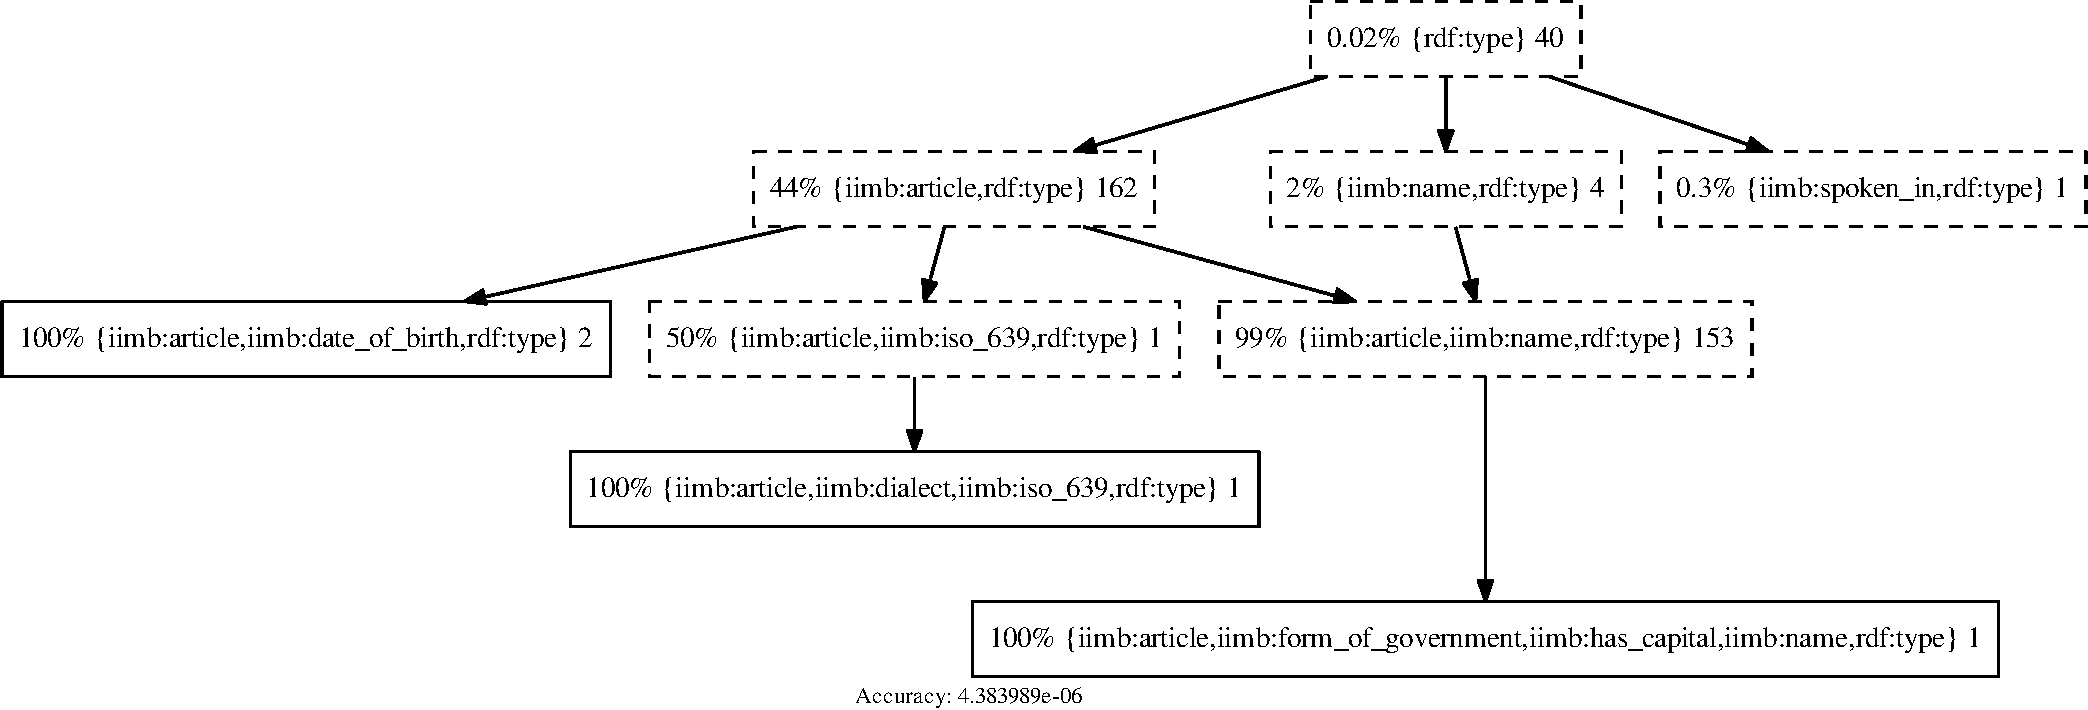
\includegraphics[width=\textwidth]{iimb_approximation_example_crop}
\caption{
  An example of a discernibility partition for an identity relation
    consisting of 365 pairs applied to the fourth IIMB linkset.
  Each node is annotated with the set of predicates $P$ for which
    its pairs are $P$-indiscernible.
  The number of identity pairs within each partition set
    is displayed to the right of the predicate set label.
  Partition sets that contain no identity pair are not show.
  The number that occurs to the left of the predicate label in each node
    indicates how may pairs in that node are identity pairs.
  The lower approximation consists of the nodes with a solid border,
    indicating that they contain only identity pairs.
  The higher approximation consists of all displayed nodes.}
\end{figure*}
\end{comment}
